\subsubsection{Маска отступа}
\label{gapMask}

Определяет стороны с которых будет отступ от объекта до других объектов.\\
Так же генератор не будет присоединять горы.\\
Доступно для столиц и городов.\\\\
Значение задается суммой сторон по схеме:

\begin{figure}[H]
\center
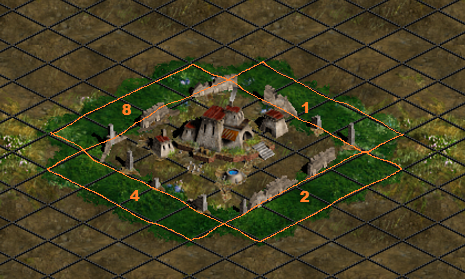
\includegraphics[width=.8\linewidth]{docImages/gapMask1.png}
\caption{Схема маски отступа}
\end{figure}

\begin{itemize}
\item \texttt{gapMask} - Диапазон [0:15], по умолчанию 0.
\end{itemize}

Пример:
\begin{figure}[H]
\lstinputlisting{docExamples/gapMask1.lua}
\end{figure}